%%%%%%%%%%%%%%%%%%%%%%%%%%%%%%%%%%%%%%%%%%%%%%%%%%%%%%%%%%%%%%%%%%%%%%
% LaTeX Example: Project Report
%
% Source: http://www.howtotex.com
%
% Feel free to distribute this example, but please keep the referral
% to howtotex.com
% Date: March 2011 
% 
%%%%%%%%%%%%%%%%%%%%%%%%%%%%%%%%%%%%%%%%%%%%%%%%%%%%%%%%%%%%%%%%%%%%%%
% How to use writeLaTeX: 
%
% You edit the source code here on the left, and the preview on the
% right shows you the result within a few seconds.
%
% Bookmark this page and share the URL with your co-authors. They can
% edit at the same time!
%
% You can upload figures, bibliographies, custom classes and
% styles using the files menu.
%
% If you're new to LaTeX, the wikibook is a great place to start:
% http://en.wikibooks.org/wiki/LaTeX
%
%%%%%%%%%%%%%%%%%%%%%%%%%%%%%%%%%%%%%%%%%%%%%%%%%%%%%%%%%%%%%%%%%%%%%%
% Edit the title below to update the display in My Documents
%\title{Project Report}
%
%%% Preamble
\documentclass[paper=a4, fontsize = 12pt]{scrartcl}
\usepackage[T1]{fontenc}
\usepackage{fourier}
\usepackage{caption}
\usepackage{subcaption}
\usepackage{lmodern}
\usepackage{float}
% (2) specify encoding
\usepackage[T1]{fontenc}

% (3) load symbol definitions
\usepackage{textcomp}

\usepackage[english]{babel}															% English language/hyphenation
\usepackage[protrusion=true,expansion=true]{microtype}	
\usepackage{amsmath,amsfonts,amsthm} % Math packages
\usepackage[pdftex]{graphicx}	
\usepackage{url}
\usepackage{comment}
\usepackage[utf8]{inputenc}
\usepackage{graphicx}
\makeatletter
\setlength{\@fptop}{0pt}
\makeatother

%%% Custom sectioning
\usepackage{sectsty}

\allsectionsfont{\centering \normalfont\scshape}


%%% Custom headers/footers (fancyhdr package)
\usepackage{fancyhdr}
\pagestyle{fancyplain}
\fancyhead{}											% No page header
\fancyfoot[L]{}											% Empty 
\fancyfoot[C]{}											% Empty
\fancyfoot[R]{\thepage}									% Pagenumbering
\renewcommand{\headrulewidth}{0pt}			% Remove header underlines
\renewcommand{\footrulewidth}{0pt}				% Remove footer underlines
\setlength{\headheight}{13.6pt}


%%% Equation and float numbering
\numberwithin{equation}{section}		% Equationnumbering: section.eq#
\numberwithin{figure}{section}			% Figurenumbering: section.fig#
\numberwithin{table}{section}				% Tablenumbering: section.tab#


%%% Maketitle metadata
\newcommand{\horrule}[1]{\rule{\linewidth}{#1}} 	% Horizontal rule

\title{
		%\vspace{-1in} 	
		\usefont{OT1}{bch}{b}{n}
		\normalfont \normalsize \textsc{Indian Institute of Technology, Delhi} \\ [25pt]
		\horrule{0.5pt} \\[0.4cm]
		\normalfont \huge \textsc{COP290}  \\

		\normalfont \normalsize \textsc{\\ Task1: Traffic density estimation using OpenCV functions} \\
		\normalfont \normalsize \textsc{\\ Subtask3: Understanding and analyzing trade-offs in software design} \\
		\horrule{2pt} \\[0.5cm]
}
\author{
		\normalfont 								\normalsize
		Abhishek Kumar (2019CS10458) \\ [-3pt]		\normalsize
        Abhinav Singhal (2019CS50768) 	
%        \today
}
\date{\normalfont \normalsize March 31, 2021 } 











%%% Begin document
\begin{document}
\maketitle


\section{Metrics}
Some of the major design considerations are as follows: 
\begin{itemize}
    \item \textbf{Benchmark:} it is the data set on which we analyze the trade-offs. The video that we used for Assignment 1 part(b), is our benchmark for Assignment 1 part(c). 
    
    \item \textbf{Baseline:} it is the method against which we compare other methods/parameters, and see whether we are getting a better or worse trade-off. Our Assignment 1 part(b) code is the baseline for Assignment 1 part(c). 
    
    \item \textbf{Utility - Run-time Trade-Off Analysis:} for both queue density and dynamic density (using optical flow) has been performed and the utility metric is defined as follows- for each of queue density and dynamic density error estimation, we take the RMS value of the difference in values of a method with respect to the baseline over all the frames and divide by RMS value of the baseline over all the frames to get the error. 
    
    \item \textbf{Running Time and CPU Performance:} used 'chrono::high\textunderscore{}resolution\textunderscore{}clock' to measure the time taken for the entire method to complete and store the total execution times separately for the various methods. We have used System Monitor available in Ubuntu to analyze CPU usage. 
    
\end{itemize}













\section{METHODS}
Here we discuss the various methods implemented and with what parameters:
\begin{itemize}
    \item \textbf{Method 1: sub-sampling frames -} This method also analyzes queue density and dynamic density similar to Assignment 1 part (b) with slight modification - it takes a parameter 'x' ,i.e., how many frames to drop in between. So we process every 'x' frame i.e. process frame N and then frame N+x, and for all intermediate frames we just use the value obtained for N. In this method we expect the total processing time to reduce, and utility to decrease as intermediate frames values would differ from baseline.
    
    \item \textbf{Method 2: Background Subtraction vs Optical Flow -} with the help of this method we compare the results of Dynamic density calculated using two algorithms - Background Subtraction and Dense Optical Flow, (where the dense optical flow is our baseline). Clearly, we can expect error to be somewhat higher with respect to background subtraction because it is a much less sophisticated algorithm as compared to dense optical flow using the 'calcOpticalFlowFarneback' algorithm.
    
    \item \textbf{Method 3: reduced resolution of frames -} We give the width and height as the parameters to this method which will lower the resolution of each frame before calculating the queue and dynamic densities. Here we expect lower resolution frames to be processed faster, but having higher errors.
    
    \item \textbf{Method 4: split spatially across threads -} Here the number of threads is given as an argument and accordingly each thread is given a vertically cropped section (roughly equal area for each thread) of the video to process. We can expect very high error in this method because upon dividing the area, the dense optical flow algorithm would be greatly disturbed and hence produce inaccurate results.
    
    \item \textbf{Method 5: split temporally across threads -} Similar to method 4, here also we give the number of threads as an argument, but the difference is that instead of splitting work spatially, we distribute it temporally across the various threads, i.e., we give consecutive frames to different threads for processing. For example, if there are two threads, then the first half of the video is given to the first thread and the second half is given to the second thread and so on.

\end{itemize}

Apart from the respective parameters for the respective methods, all methods take in an additional argument called 'queueLength' which is used to get more accurate results while calculating optical flow using the 'calcOpticalFlowFarneback' algorithm. Though all frames are processed sequentially (except in Method -1), the optical flow is calculated between the frames separated by queueLength (5 for all methods) distance. This had to be implemented because otherwise if optical flow is calculated between consecutive frames, then dynamic density keeps flickering and drops to zero with very high freqency (maybe due to very less movement of vehicles from one frame to another). As a result the entire graph would be skewed. Processing optical flow with respect to frames at a distance ensures that optical flow doesn't drop to zero, when not needed.








\section{TRADE-OFF ANALYSIS}

In this section, the four points that user will press which are used for warping the frames are kept constant throughout the execution of all methods in order to reduce human errors in trade off analysis.
\subsection{The Baseline}
The following graph shows the baseline graphs of queue densities and dynamic densities from which we will be calculating deviations and errors for the various methods. \\

\begin{figure}[ht!]
    \centering
    \captionsetup{justification=centering,margin=2cm}
    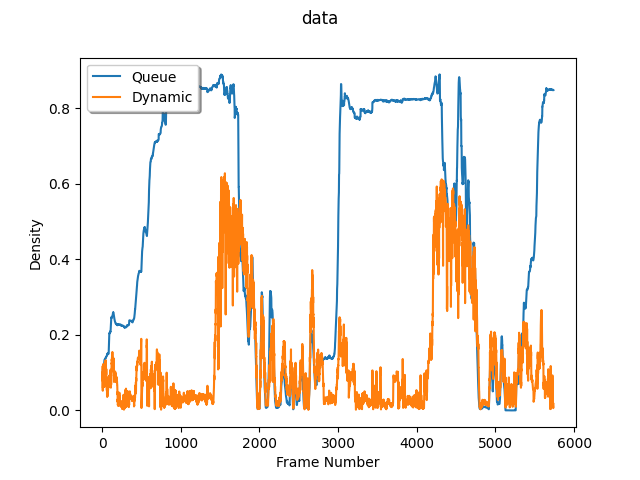
\includegraphics[width=15cm]{data.png}
    \caption{ Assignment 1 part (b)\\Total Runtime = 428 seconds}
    \label{fig:baseline}
\end{figure}




\subsection{Method - 1}
Figure 3.2 shows a typical output of Method - 1 wherein we have set x = 10 ( i.e, after processing Nth frame, we process N + 10Th frame). Figure 3.3 and 3.4 show the error vs run-time plot for various values of x, from which we can derive interesting conclusions. 

\begin{figure}[H]
    \centering
    \captionsetup{justification=centering,margin=2cm}
    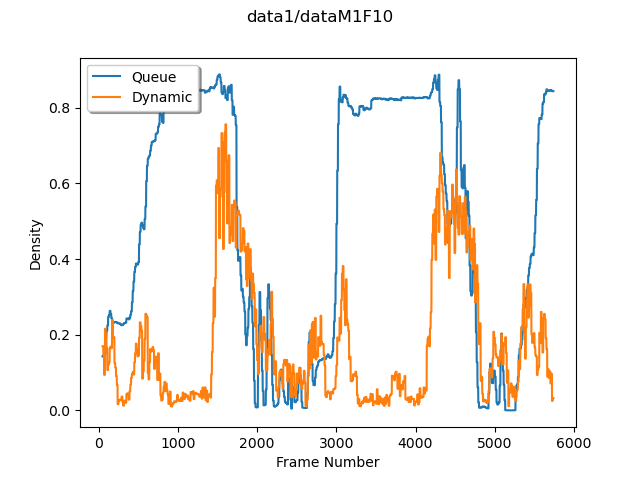
\includegraphics[width=15cm]{dataM1F10.png}
    \caption{ Method - 1: x = 10 \\Total Runtime = 65 seconds}
    \label{fig:typicalM1}
    
     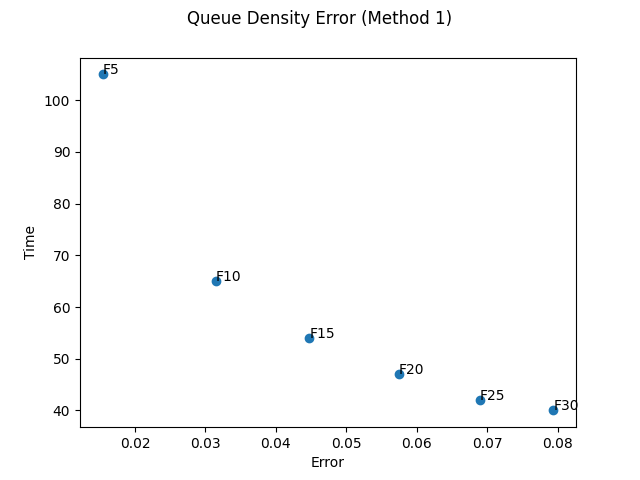
\includegraphics[width=15cm]{method1_tradeoff_queue.png}
    \caption{ Method - 1: Queue Density Trade-Off}
    \label{fig:M1QueueTradeOff}

\end{figure}

\begin{figure}[H]
    \centering
    \captionsetup{justification=centering,margin=2cm}
    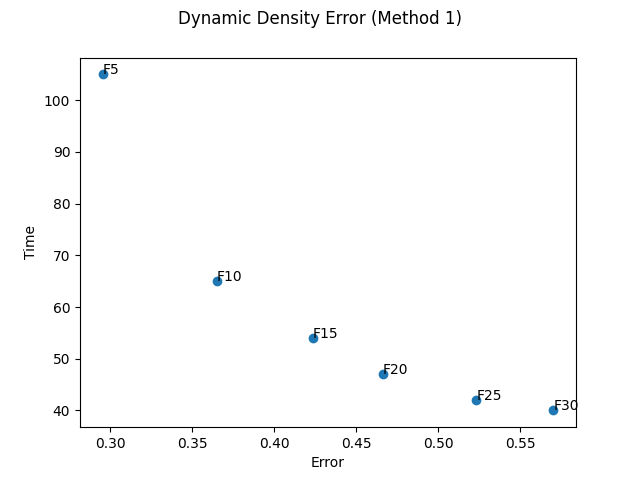
\includegraphics[width = 15cm]{method1_tradeoff_dynamic.png}
    \caption{Method - 1: Dynamic Density Trade-Off}
    \label{fig:M1DynamicTradeOff}
\end{figure}

\paragraph{Observations:}
\begin{itemize}
    \item [[Fig 3.2]] The queue and dynamic density curves seem a little grainier and somewhat more discrete as compared to the baseline. This is so because we are skipping 9 in between the Nth and N+10Th frame and substituting the Nth frame's values of queue and dynamic densities for the skipped frames.
    
    \item [[Fig 3.3]] As we increase the number of frames skipped from 5 to 30, the time taken naturally decreases as we have to process less frames in the entire video and since the gap between the frames increases, the error in background subtraction also increases. We also see the concept of "diminishing returns" in action, i.e., the decrease in running time itself keeps on reducing (time gap between F5 and F10 is much larger as compared to F25 and F30). 
    
    \item [[Fig 3.4]] Overall dynamics of the graph remains same as Fig 3.3 except for the fact that the scale of error is 10 times the scale of error for queue density. The error is comparatively higher while computing optical flow because if we skip some in between frames, the 2-D vector field generated of minute displacement of individual pixels by 'calcOpticalFlowFarneback' algorithm is greatly affected as displacement of pixels is very different and changes quite a lot upon skipping frames.
\end{itemize}








\subsection{Method - 2}

The following figure shows queue and dynamic density (using background subtraction only). We observe that the error in dynamic density will be very high because it doesn't peak as much as the baseline. (All the error analysis for this method is at the end when comparing with other methods).

\begin{figure}[H]
    \centering
    \captionsetup{justification=centering,margin=2cm}
    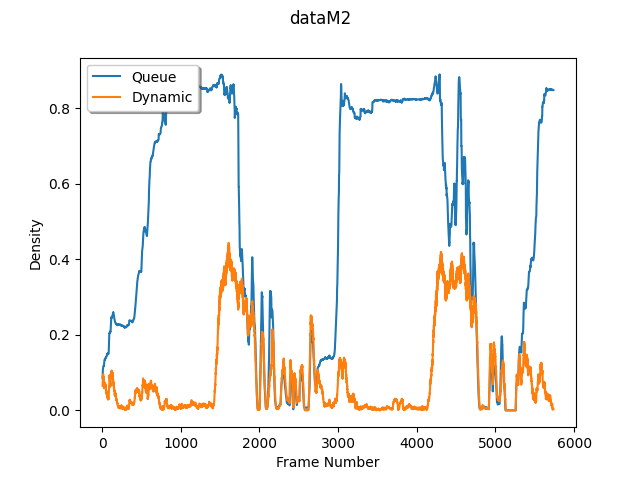
\includegraphics[width = 15cm]{dataM2.png}
    \caption{Method - 2: Dynamic Density with Background Subtraction}
    \label{fig:M2DynamicBS}
\end{figure}

\subsection{Method - 3}

Fig 3.6 and 3.7 show how time taken decreases and the error increases upon decreasing the resolution of the frames of the video. As we reduce the resolution the amount of work to be done reduces because number of pixels to be processed by the algorithms is significantly reduced at each reduction. \\
Here also we observe the concept of "diminishing returns" in action, i.e., the decrease in time taken for every reduction in quality itself decreases. As in method - 1, we would like to emphasize that error scale for queue density is of the order of 10\textsuperscript{-3} whereas for dynamic density it is 10\textsuperscript{-1} (optical flow is affected much more because upon dividing the area, the effectiveness of pixel tracking mechanism of the algorithm reduces).


\begin{figure}[H]
    \centering
    \captionsetup{justification=centering,margin=2cm}
    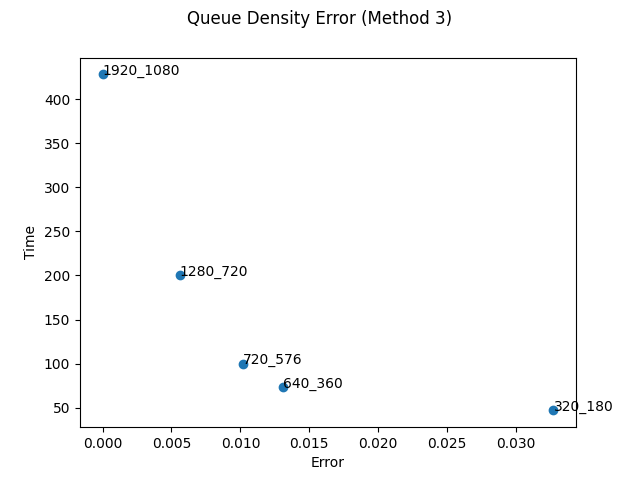
\includegraphics[width = 15cm]{method3_tradeoff_queue.png}
    \caption{Method - 3: Queue Density Trade-Off}
    \label{fig:M2QueueTradeOff}
    
    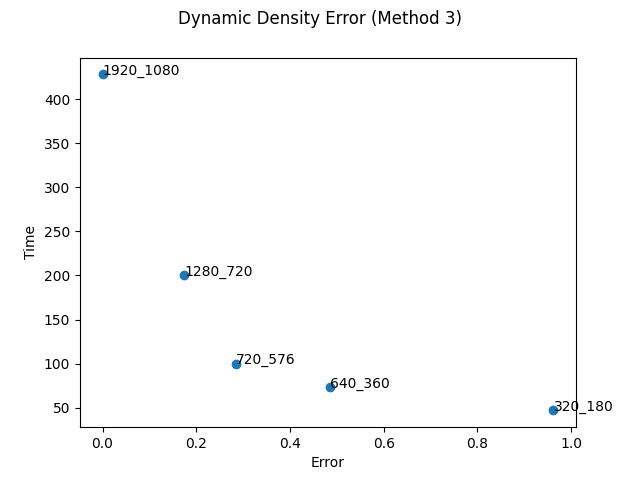
\includegraphics[width = 15cm]{method3_tradeoff_dynamic.png}
    \caption{Method - 3: Dynamic Density Trade-Off}
    \label{fig:M3DynamicTradeOff}
\end{figure}






\subsection{Method - 4}
The overall trend upon varying the number of threads from 1 to 9 while distributing the work spatially in method - 4 is depicted by figures 3.8 and 3.9 as shown below and fig 3.10 - 3.12 show the CPU and memory performance.

\begin{figure}[H]
    \centering
    \captionsetup{justification=centering,margin=2cm}
    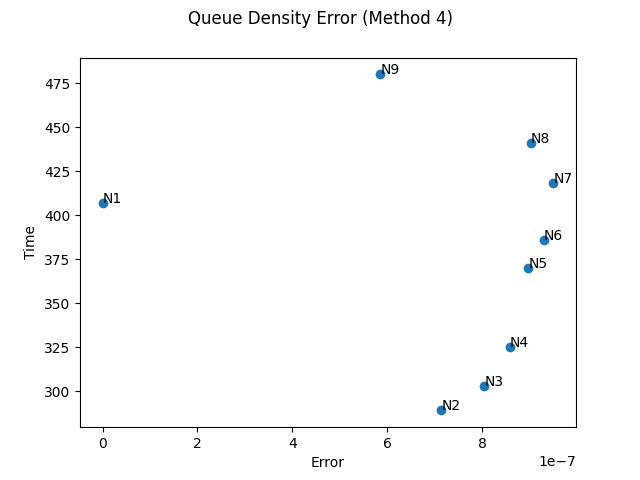
\includegraphics[width = 15cm]{method4_tradeoff_queue.png}
    \caption{Method - 4: Queue Density Trade-Off}
    \label{fig:M4QueueTradeOff}
\end{figure}
N1 is our baseline (i.e., single threaded). From both the figures we can conclude that: 

\begin{itemize}
    \item As we increase the number of threads, the area given to each thread reduces and hence, since each thread now has to do less work, which implies that the time taken is less as compared to the baseline and the error increases because if you divide the area, the algorithms don't work properly. This holds true for the first few trials. From 3 threads and on-wards, the time taken increases instead of decreasing and surprisingly after 6 threads, it exceeds the time taken by baseline. The exact reason for this counter-intuitive phenomenon is explained later on in the concluding section at the end.
    
    \item Similar results for dynamic density also, but the magnitude of error is higher as explained earlier also.
    
\end{itemize}


\begin{figure}[H]
    \centering
    \captionsetup{justification=centering,margin=2cm}
    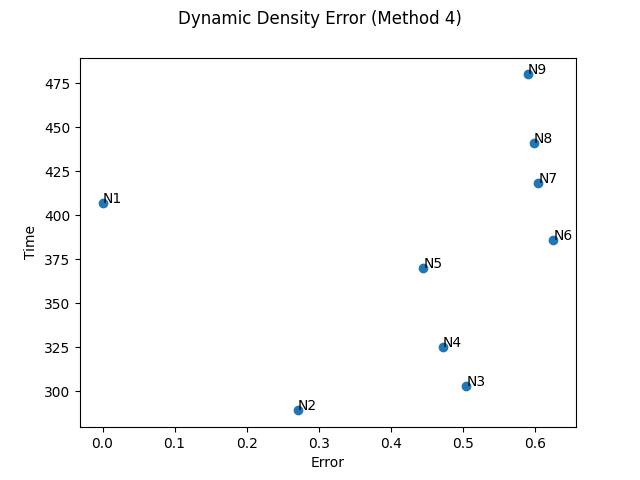
\includegraphics[width = 15cm]{method4_tradeoff_dynamic.png}
    \caption{Method - 4: Dynamic Density Trade-Off}
    \label{fig:M4DynamicTradeOff}
    
    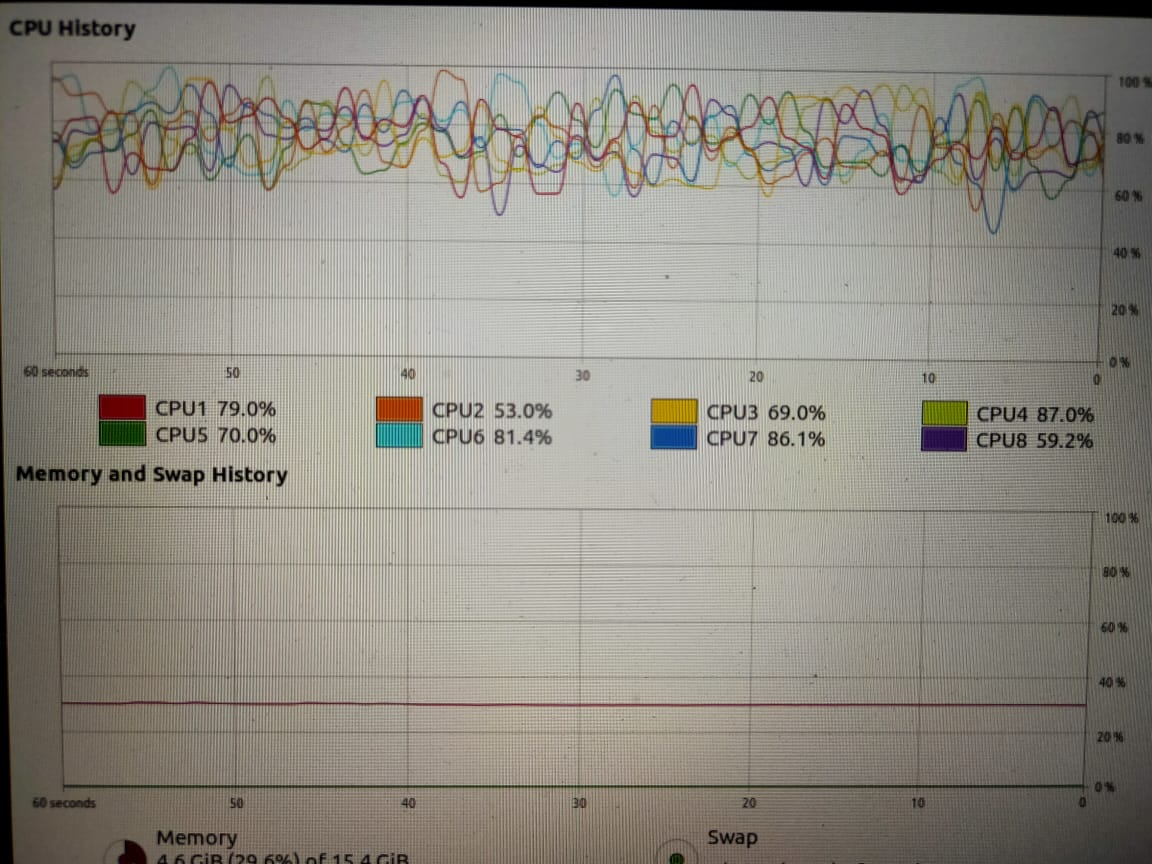
\includegraphics[width = 14cm]{4_4.jpeg}
    \caption{M - 4: CPU and Memory Performance at 4 threads}
    \label{fig:M4CPUT4}
\end{figure}

\begin{figure}[H]
    \centering
    \captionsetup{justification=centering,margin=2cm}
    
    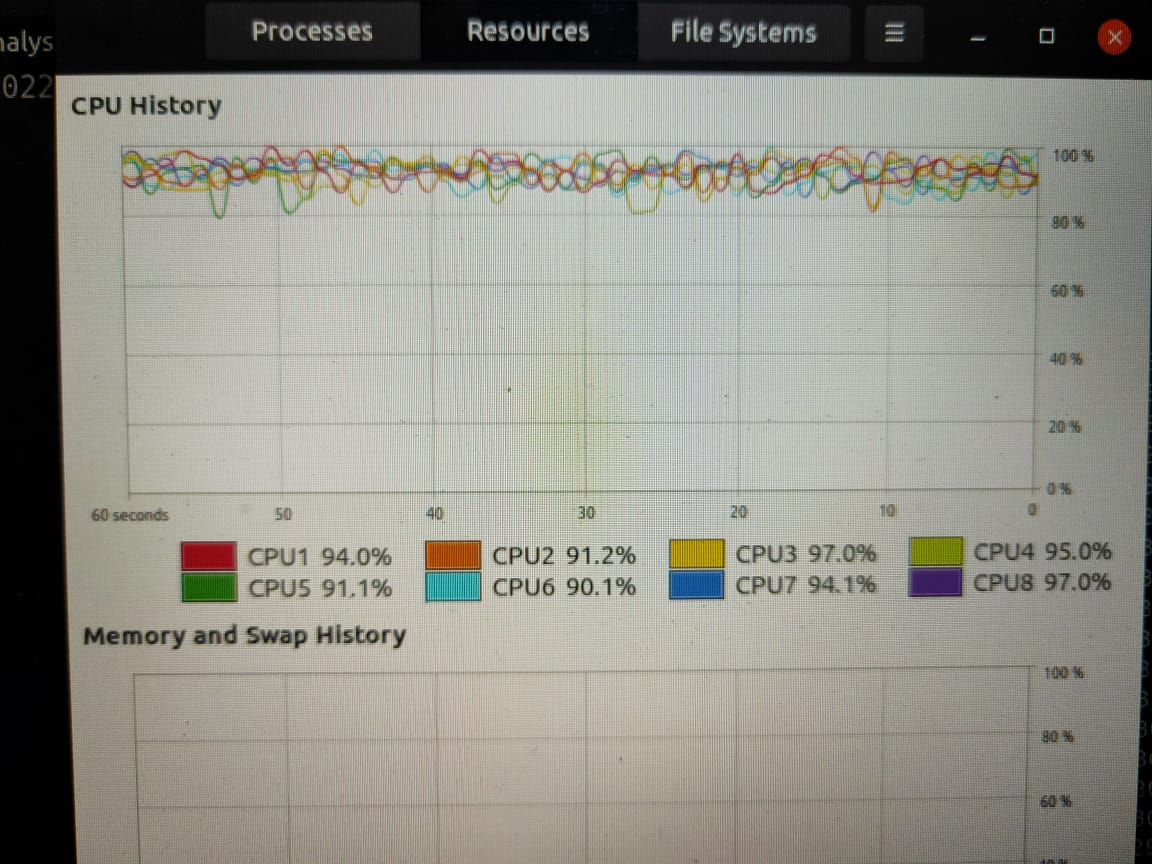
\includegraphics[width = 14cm]{4_6.jpeg}
    \caption{M - 4: CPU and Memory Performance at 6 threads}
    \label{fig:M4CPUT6}
    
    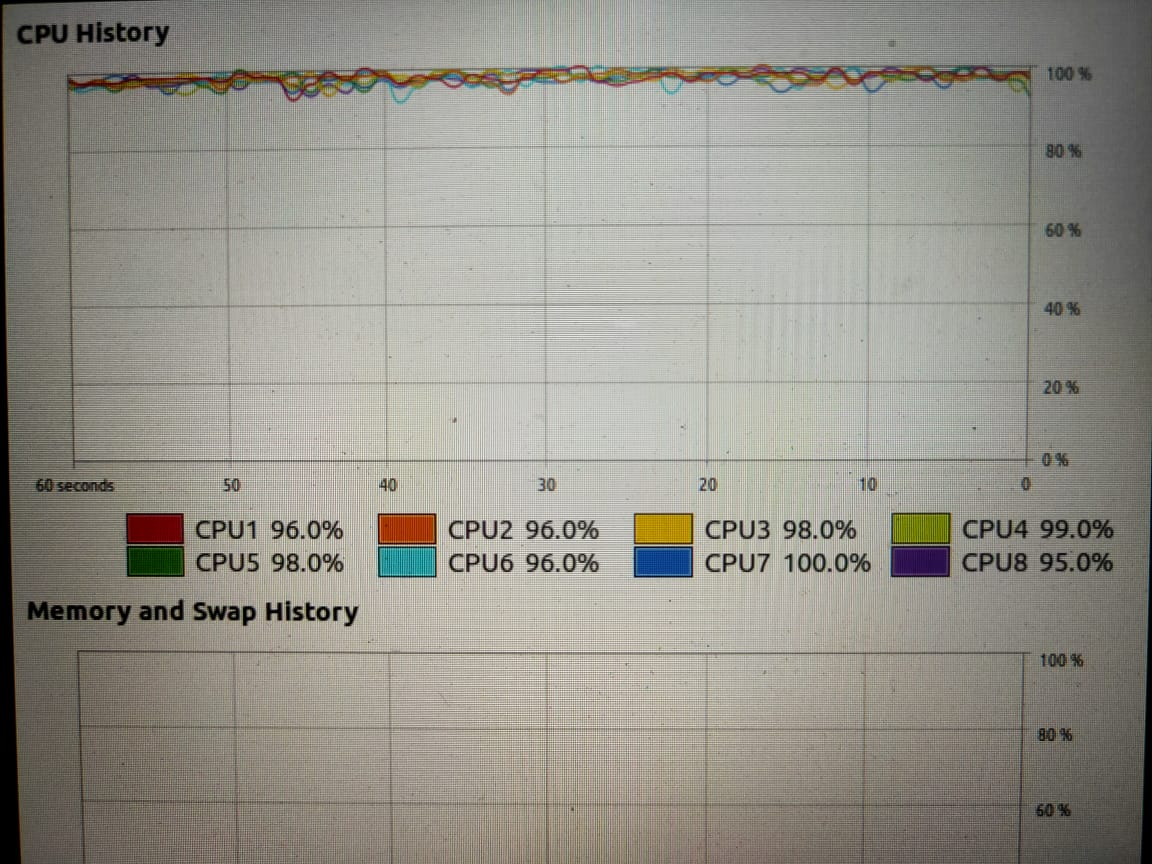
\includegraphics[width = 14cm]{4_8.jpeg}
    \caption{M - 4: CPU and Memory Performance at 8 threads}
    \label{fig:M4CPUT6}
\end{figure}

From figures 3.10 - 3.12 we observe that: 
\begin{itemize}
    \item explain here!
    
    \item explain here!
    
    \item explain here!
\end{itemize}






\subsection{Method - 5}

Here, the queue and dynamic density graph is not shown as it is very similar to the baseline. This is so because we are temporally splitting the work among the threads. Hence, except at the abrupt end frames of the various threads, the graph will be same as baseline and error is present only at those discontinuities. \\ \\
Fig 3.13 and 3.14 show the queue density and dynamic density graphs respectively and Fig 3.15-3.17 show CPU and Memory utilization for method - 5.\\ \\

We observe that \\\\
Explain after above explanation is done (analyze space accordingly)\\ \\ 
*** Time taken should have increased after 5 or 6 threads but it remains constant?!?!

\begin{figure}[H]
    \centering
    \captionsetup{justification=centering,margin=2cm}
    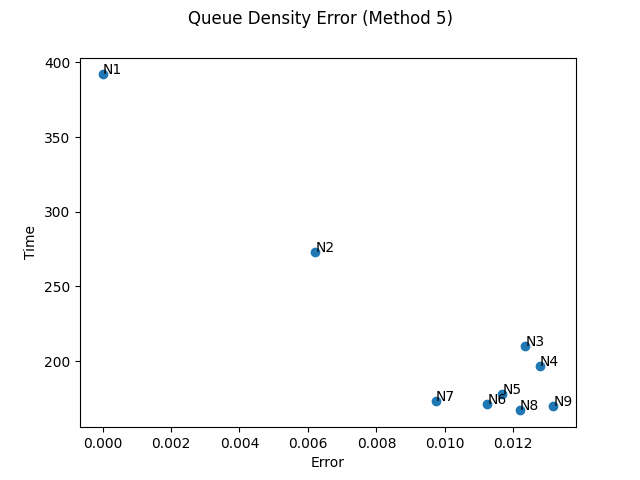
\includegraphics[width = 15cm]{method5_tradeoff_queue.png}
    \caption{Method - 5: Queue Density Trade-Off}
    \label{fig:M5QueueTradeOff}
    
    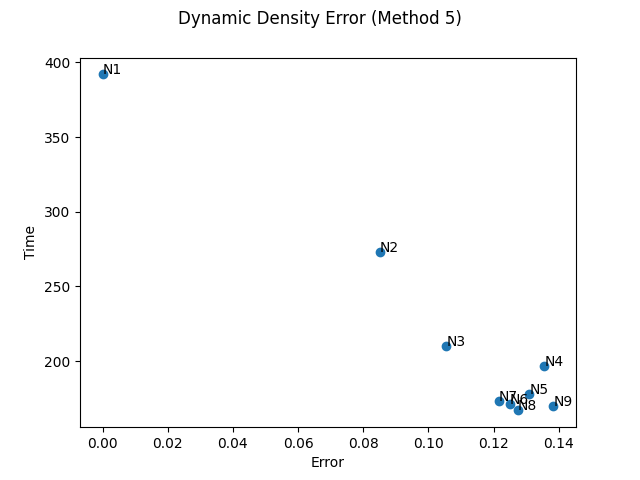
\includegraphics[width = 15cm]{method5_tradeoff_dynamic.png}
    \caption{Method - 5: Dynamic Density Trade-Off}
    \label{fig:M5DynamicTradeOff}
\end{figure}

\begin{figure}[H]
    \centering
    \captionsetup{justification=centering,margin=2cm}
    
    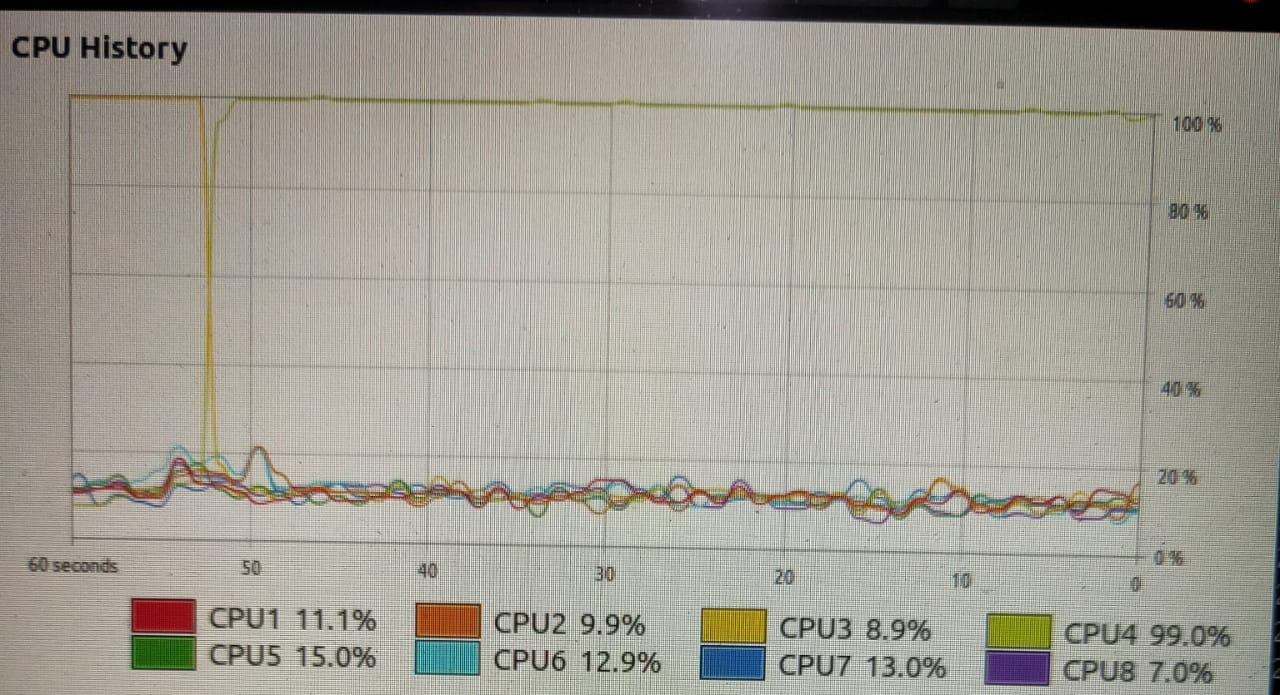
\includegraphics[width = 14cm]{5_1.jpeg}
    \caption{M - 5: CPU Performance at 1 thread}
    \label{fig:M5CPUT1}
    
    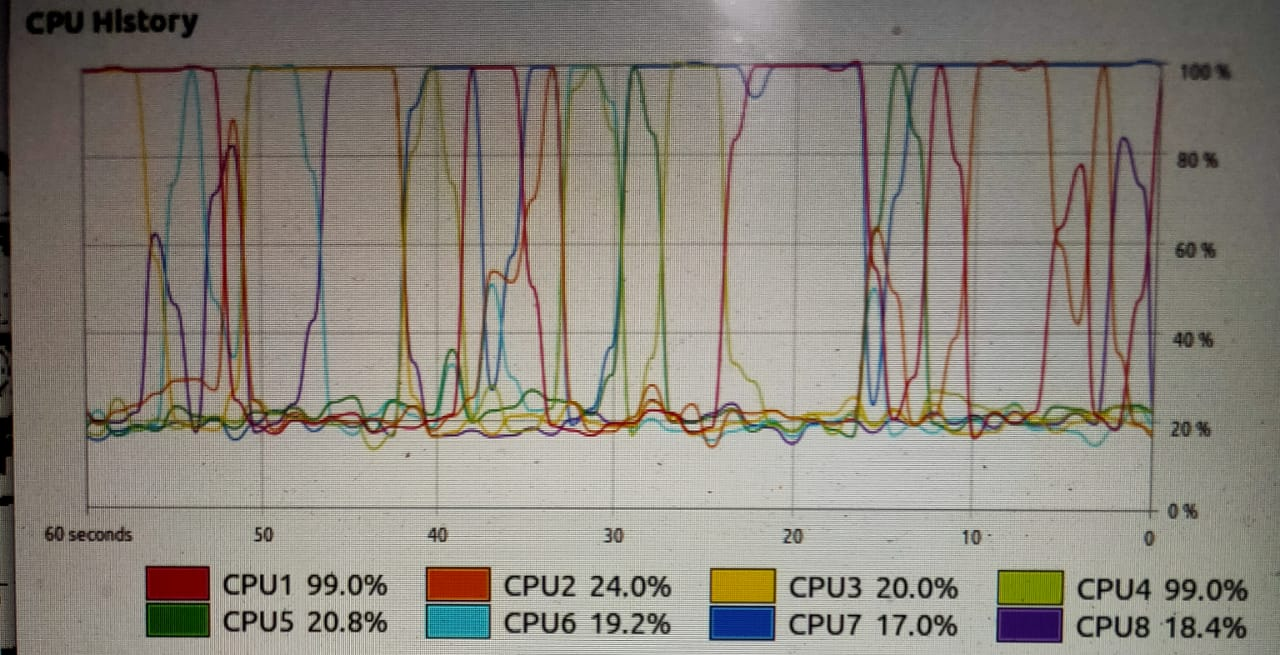
\includegraphics[width = 14cm]{5_2.jpeg}
    \caption{M - 5: CPU Performance at 2 threads}
    \label{fig:M5CPUT2}
    
    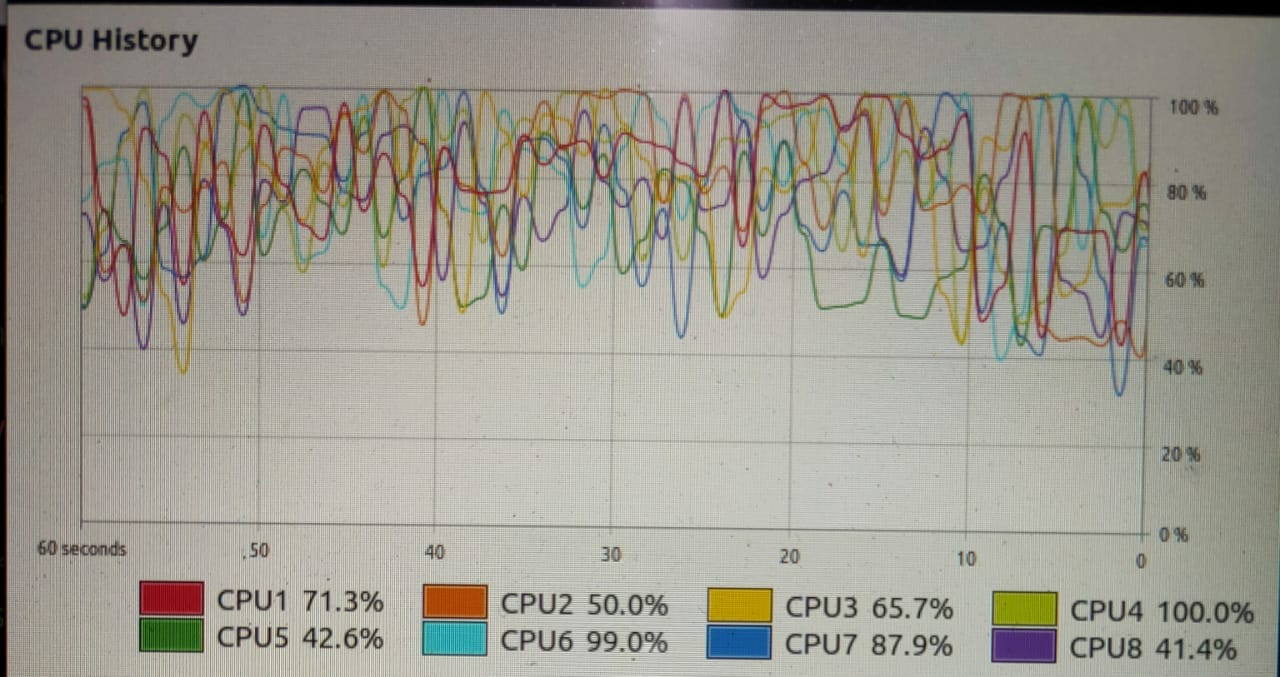
\includegraphics[width = 14cm]{5_4.jpeg}
    \caption{M - 5: CPU Performance at 4 threads}
    \label{fig:M5CPUT4}
\end{figure}

From figures 3.15 - 3.17 we observe that: 
\begin{itemize}
    \item explain here!
    
    \item explain here!
    
    \item explain here!
\end{itemize}


\section{Deriving Conclusions and Insights}

\subsection{Why performance decrease on increasing too many threads?}

Initially it might seem that if little threading boosts our performance, then a lot of threading would be even better. But it isn't so - In fact, we observed that using too many threads slows down the program after a limit. \\

There are two main reasons why performance bogs down - Splitting the given work among too many threads results in too little work per thread and hence the overhead of initiating and terminating threads itself slows down the CPU and disguises the actual work, and another overhead which costs the CPU is from the way the multiple threads share the finite hardware resources.\\

First, We must understand that threads are of two kinds - software threads (which are created by programs) and hardware threads (which are actually physically present and is an hardware resource). It is possible that there be one or more hardware thread per core in a chip.\\

When there are more software threads than hardware threads, the operating system typically resorts to round robin scheduling. Each software thread gets a short turn, called a time slice, to run on a hardware thread. When the time slice runs out, the scheduler suspends the thread and allows the next thread waiting its turn to run on the hardware thread. Time slicing ensures that all software threads make some progress. Otherwise, some software threads might hog all the hardware threads and starve other software threads. However, fair distribution of hardware threads incurs overhead. \\

A significant overhead of time slicing is saving and restoring a thread's cache state, which can be megabytes. Modern processors rely heavily on cache memory, which can be about 10 to 100 times faster than main memory. Accesses that hit in cache are not only much faster; they also consume no bandwidth from the memory bus. Caches are fast, but finite. When the cache is full, a processor must evict data from the cache to make room for new data. Typically, the choice for eviction is the least recently used data, which is typically data from an earlier time slice. Thus software threads tend to evict each other's data, and the cache fighting from too many threads can hurt performance.\\

A similar overhead, at a different level, is thrashing virtual memory. Most computers use virtual memory. Virtual memory resides on disk, and the frequently used portions are kept in real memory. Similar to caches, the least recently used data is evicted from memory to disk when necessary to make room. Each software thread requires virtual memory for its stack and private data structures. As with caches, time slicing causes threads to fight each other for real memory and thus hurts performance. In extreme cases, there can be so many threads that the program runs out of even virtual memory.[1] 

\subsection{So Which Method is the Best?}

Now we try to compare all the 5 methods. To get a single value for each method to be compared, we take the average value of all the trials of that method. for example, to get a single value for method 1, we compute the average error and running time for the 6 trials that were considered - 5, 10, 15, 20, 25 and 30 frames skipped. Similarly for the other methods. The following two plots try to summarize the picture.
\\\\
*** fill remaining explanation here after explanation on page 14.\\
*** Method 2 ka time queue density mein itna kam kyun hai?

\begin{figure}[H]
    \centering
    \captionsetup{justification=centering,margin=2cm}
    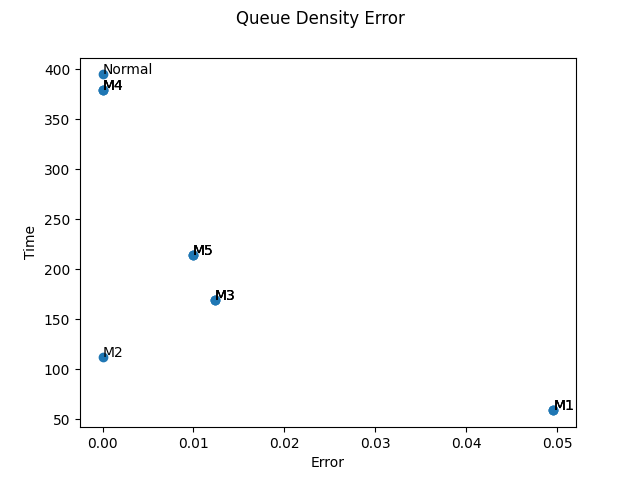
\includegraphics[width = 15cm]{tradeoff_queue.png}
    \caption{All Methods: Queue Density Trade-Off}
    \label{fig:AllMQueueTradeOff}
    
    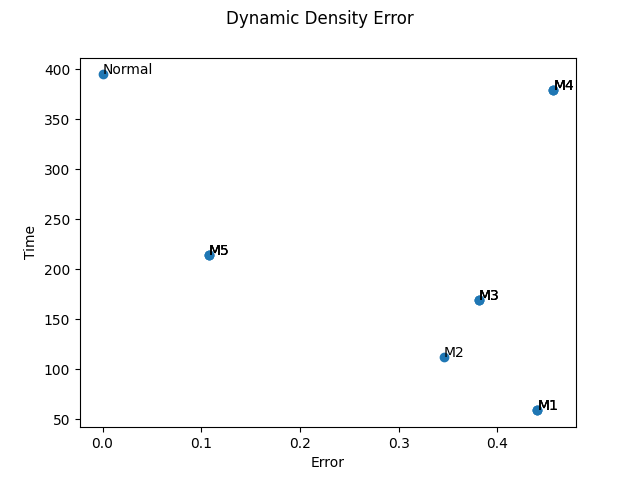
\includegraphics[width = 15cm]{tradeoff_dynamic.png}
    \caption{All Methods: Dynamic Density Trade-Off}
    \label{fig:AllMDynamicTradeOff}
\end{figure}

\section{References}

\begin{itemize}
    \item [[1]]   https://www.codeguru.com/cpp/sample\textunderscore{}chapter/article.php/c13533/Why-Too-Many-Threads-Hurts-Performance-and-What-to-do-About-It.htm\#:\sim:text=Modern\%\\20processors\%20rely\%20heavily\%20on,times\%20faster\%20than\%20main\%20memory.\\\&text=Thus\%20software\%20threads\%20tend\%20to,level\%2C\%20is\%20thrashing\%20\\virtual\%20memory.
\end{itemize}\\\\\\\\\\\\\\\\\\\\\\\\\\\\\\\\\\\



\centerline{\huge  \sim THANK YOU \sim }








%%% End document
\end{document}
